% Propietario conservado: /Users/ruben/Documents/New project/output/REVISION_ARGUMENTAL_APERTURAS_CIERRES_20260915/VI/delivery/MANUSCRIPT_VI_ES_EN_COMPLETE/source_es/sections/04_atlas_familias.tex
\section{Classification des sections persistantes et de leurs observables internes}
\label{vi:vi:sec:atlas}

La classification commence dans le support sur lequel agit le transport.
Les noms physiques s’interprètent après la construction de leurs invariants.
Cette priorité permet de distinguer une position, une histoire et une espèce :
la position appartient à l’atlas fini ; l’histoire conserve les transitions
qui la produisent ; le type de persistance réunit des histoires compatibles avec une
même classification. Une masse évaluée est une lecture ultérieure de cet objet.

\subsection{Parité, profondeur et multisections}

Sur la copie positionnelle d’APP, on considère
\[
 I_9=\{1,\ldots,9\},\qquad \mathcal C=I_9\times I_9.
\]
La paire ordonnée conserve les deux axes. Nous définissons le classificateur de parité
\[
 f(r,c)=
 \begin{cases}
 \ell,&r,c\text{ impairs},\\
 \nu,&r\text{ impair},\ c\text{ pair},\\
 d,&r\text{ pair},\ c\text{ impair},\\
 u,&r,c\text{ paires},
 \end{cases}
 \qquad g(r,c)=\max\{|r-5|,|c-5|\}.
\]
Les symboles de la première application nomment initialement des classes internes.
La seconde mesure la profondeur combinatoire par rapport au centre. L’association
ultérieure à des secteurs physiques doit conserver ces définitions.


% BEGIN OWNER /Users/ruben/Documents/New project/output/REVISION_ARGUMENTAL_APERTURAS_CIERRES_20260915/VI/delivery/MANUSCRIPT_VI_ES_EN_COMPLETE/source_es/figures/atlas_clasificacion.tex
\begin{figure}[H]
\centering
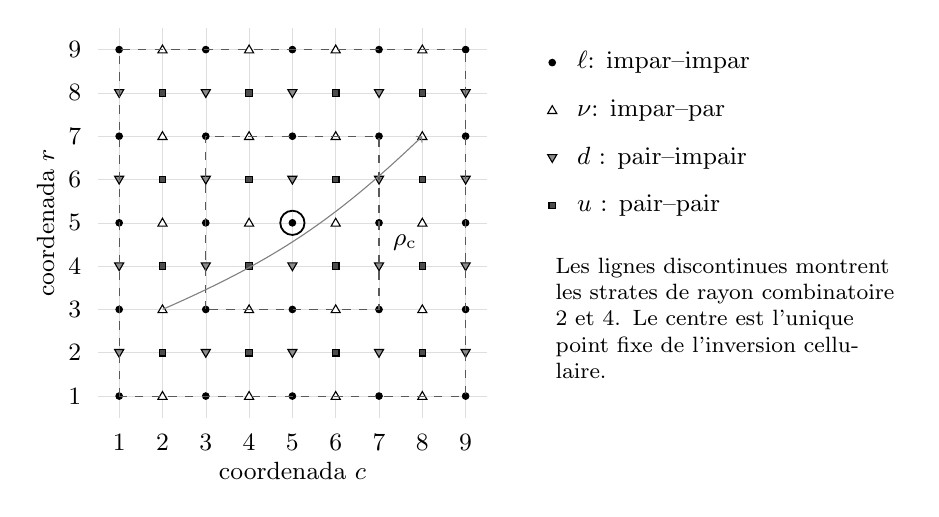
\begin{tikzpicture}[x=.55cm,y=.55cm, every node/.style={font=\small}]
  \draw[step=1,black!13,very thin] (.5,.5) grid (9.5,9.5);
  \foreach \k in {1,...,9} {
    \node[below] at (\k,.35) {$\k$};
    \node[left] at (.35,\k) {$\k$};
  }
  \node[below] at (5,-.3) {coordenada $c$};
  \node[rotate=90] at (-.7,5) {coordenada $r$};
  \foreach \r in {1,...,9} {
    \foreach \c in {1,...,9} {
      \pgfmathtruncatemacro{\pr}{mod(\r,2)}
      \pgfmathtruncatemacro{\pc}{mod(\c,2)}
      \ifnum\pr=1
        \ifnum\pc=1
          \draw[fill=black] (\c,\r) circle (.075);
        \else
          \draw[fill=white] (\c,\r+.105)--(\c-.105,\r-.075)--(\c+.105,\r-.075)--cycle;
        \fi
      \else
        \ifnum\pc=1
          \draw[fill=black!45] (\c,\r-.105)--(\c-.105,\r+.075)--(\c+.105,\r+.075)--cycle;
        \else
          \draw[fill=black!70] (\c-.075,\r-.075) rectangle (\c+.075,\r+.075);
        \fi
      \fi
    }
  }
  \draw[black!65,dashed] (3,3) rectangle (7,7);
  \draw[black!65,dashed] (1,1) rectangle (9,9);
  \draw[line width=.65pt] (5,5) circle (.28);
  \draw[->,black!50] (2,3) to[bend right=10] (8,7);
  \node[fill=white,inner sep=2pt] at (7.6,4.55) {$\rho_{\mathrm c}$};
  \begin{scope}[shift={(11,8.7)}]
    \draw[fill=black] (0,0) circle (.075);
    \node[right] at (.35,0) {$\ell$: impar--impar};
    \draw[fill=white] (0,-.995)--(-.105,-1.175)--(.105,-1.175)--cycle;
    \node[right] at (.35,-1.1) {$\nu$: impar--par};
    \draw[fill=black!45] (0,-2.305)--(-.105,-2.125)--(.105,-2.125)--cycle;
    \node[right] at (.35,-2.2) {$d$ : pair--impair};
    \draw[fill=black!70] (-.075,-3.375) rectangle (.075,-3.225);
    \node[right] at (.35,-3.3) {$u$ : pair--pair};
    \node[anchor=west,text width=4.4cm,align=left,font=\footnotesize]
      at (-.15,-5.9) {Les lignes discontinues montrent les strates de rayon combinatoire $2$ et $4$. Le centre est l’unique point fixe de l’inversion cellulaire.};
  \end{scope}
\end{tikzpicture}
\caption[Classification sur l’atlas positionnel]{Classification sur l’atlas positionnel. Les marques distinguent les
quatre classes internes de parité, antérieures à leurs réalisations physiques.
La profondeur se mesure avec $g(r,c)=\max(|r-5|,|c-5|)$.
La flèche illustre $(2,3)\mapsto(8,7)$ sous l’inversion cellulaire ;
elle ne représente ni une trajectoire dynamique ni un changement de saveur.
Le cercle central marque $(5,5)$, de profondeur nulle.}
\label{vi:vi:fig:atlas}
\end{figure}

% END OWNER


\begin{definition}[Multisection de famille et de profondeur]
Pour chaque paire réalisée \(y=(f,g)\), on définit
\[
 \mathfrak S_y=\{(r,c)\in\mathcal C:(f(r,c),g(r,c))=y\}.
\]
Son relèvement aux états persistants est la préimage par la projection
sur l’atlas, en conservant les feuillets, les orientations et la mémoire de l’extension.
\end{definition}

\begin{proposition}[Recensement des multisections]
\label{vi:vi:prop:censo13}
L’atlas contient \(81\) cellules et exactement \(13\) multisections non vides.
Leur distribution est
\[
\begin{array}{c|c|c|r}
\text{classe}&\text{profondeurs}&\text{cardinaux}&\text{total}\\\hline
\ell&0,2,4&1,8,16&25\\
\nu&1,2,3,4&2,4,6,8&20\\
d&1,2,3,4&2,4,6,8&20\\
u&1,3&4,12&16
\end{array}
\]
\end{proposition}
\begin{proof}
Dans \(I_9\), il y a \(5\) impairs et \(4\) pairs. Les quatre classes ont pour
cardinaux \(25,20,20,16\). Pour la classe impair--impair, les carrés
centrés de rayons \(0,2,4\) contiennent \(1,9,25\) points ; les
différences sont \(1,8,16\). Pour impair--pair, les rectangles accumulés
aux rayons \(1,2,3,4\) contiennent \(2,6,12,20\) points, dont les
différences sont \(2,4,6,8\). Échanger les axes prouve le cas
pair--impair. Dans pair--pair, il y a \(4\) points jusqu’au rayon \(1\) et \(16\)
jusqu’au rayon \(3\), donc les strates ont \(4,12\) points.
Ce sont des ensembles disjoints et leur réunion est \(\mathcal C\).
\end{proof}

Ce recensement explique le sens de chaque cardinal avant tout tableau
de particules. La profondeur \(g\) ne s’identifie pas non plus à elle seule à
l’indice d’une génération physique : cette identification utilise les applications
de réalisation du secteur correspondant.

\subsection{Conjugaison centrale et sélection d’une cellule}

L’inversion cellulaire est
\[
 \rho_{\mathrm c}(r,c)=(10-r,10-c).
\]
Elle conserve la parité et la profondeur et agit donc dans chaque
multisection. Son unique point fixe satisfait \(2r=2c=10\) : c’est \((5,5)\).
Les \(80\) cellules restantes se regroupent en \(40\) paires. Il y a ainsi
\(41\) orbites, dont une seule est ponctuelle.

\begin{proposition}[Obstruction à la sélection ponctuelle non centrale]
Si l’on exige que le sélecteur d’une cellule dépende uniquement de la paire
famille--profondeur et soit équivariant pour \(\rho_{\mathrm c}\), il ne
peut exister que dans la multisection centrale.
\end{proposition}
\begin{proof}
L’inversion agit trivialement sur la paire \(y\). L’équivariance de
\(a(y)\in\mathfrak S_y\) exige
\(a(y)=a(\rho_{\mathrm c}y)=\rho_{\mathrm c}a(y)\).
Par conséquent, \(a(y)\) devrait être l’unique point fixe \((5,5)\).
Dans la multisection centrale, c’est précisément le choix disponible.
\end{proof}

La conséquence est structurelle. Le traitement de l'électron au moyen d'une
fibre de rang \(1\) n'autorise pas à traiter de cette manière toutes les autres
familles. Hors du centre, l'orbite, la multisection et les orientations
qu'elle conserve appartiennent à l'objet évalué.

\subsection{Classification des routes et mémoire positionnelle}

La carte chronologique attribue à chaque cellule le sextuplet
\[
 \mathcal R(r,c)=
 (n_A,s_C,k_{\Delta_4},b_{120},b_{\zeta},\tau_{12})_{r,c}.
\]
Les cinq coordonnées entières proviennent du registre orienté ; la dernière
conserve le mot dodécaphasique. Deux cellules appartiennent à la même famille
de routes lorsque ces six lectures coïncident. C'est un quotient différent
de celui de famille--profondeur.

Dans le recensement fini documenté de cette carte apparaissent \(56\) familles.
L'histogramme des tailles est
\[
 41\times1,\quad10\times2,\quad2\times3,\quad1\times4,\quad2\times5.
\]
Les identités
\[
 41+10+2+1+2=56,\qquad
 41+20+6+4+10=81
\]
vérifient le nombre de classes et la couverture du support. La reproduction
du recensement requiert les sextuplets produits par le transport, et pas seulement ces
deux sommes. Le dossier de données conserve les \(81\) lignes et les
\(56\) classes complètes.

L’ordre lexicographique étant fixé dans chaque fibre, soit \(\kappa_{\mathrm{pos}}\)
le rang de la cellule. Alors
\[
 (r,c)\longmapsto\bigl(\mathcal R(r,c),\kappa_{\mathrm{pos}}(r,c)\bigr)
\]
est injective. Il faut \(5\) valeurs de mémoire de position parce qu’il
existe des fibres de taille \(5\) ; le principe des tiroirs empêche un
relèvement injectif uniforme avec moins de valeurs. Cette mémoire n’est ni la couleur
ni l’exposant massique, bien que tous interviennent ensuite dans une même histoire.

\subsection{Couleur résiduelle, saveur et feuillets}

Dans les \(36\) cellules de première coordonnée paire, l’observable de couleur
résiduelle se définit par
\[
 \operatorname{col}(r,c)=r-c\pmod3.
\]
Pour chaque \(r\) pair, les \(9\) valeurs de \(c\) parcourent \(3\)
fois chaque classe. Il en résulte la répartition exacte
\[
 36=12+12+12.
\]
L’inversion centrale transforme cette observable en son opposée, car
\[
 (10-r)-(10-c)=-(r-c).
\]
Elle fixe la classe \(0\) et échange \(1\) et \(2\). La représentation
de couleur utilise ultérieurement ce support ternaire et ses opérateurs ;
le nombre de résidus ne remplace pas la construction de la représentation.

La saveur distingue les classes et les réalisations du secteur, tandis que la couleur
résiduelle distingue les positions à l’intérieur du support ternaire correspondant.
Le feuillet, en revanche, identifie l’évaluation arithmétique qui participe à
une transition. L’échange de feuillets agit sur une histoire ; ce n’est pas
une opération de changement de nom de saveur. Cette distinction permet de
formuler séparément les mélanges, les conjugaisons et les évaluations
de masse.

\subsection{Domaine des orientations de l'atlas}

Chaque cellule admet \((h,v)\in\{\pm1\}^2\), de sorte que
\[
 \mathcal C^{\mathrm{or}}=\mathcal C\times\{\pm1\}^2,
 \qquad |\mathcal C^{\mathrm{or}}|=324.
\]
L'orientation canonique de \(81\) routes et le domaine complet de \(324\)
sont deux domaines distincts. Un lecteur peut descendre à une famille dans la
première carte et cesser d'être constant lorsque les quatre
orientations sont considérées. Ainsi, chaque énoncé sur la coïncidence des lecteurs
identifie son domaine avant de publier le recensement.

La structure finie combine donc positions, familles de routes,
multisections, orbites de conjugaison et observables résiduels. Aucune
de ces partitions ne remplace les autres. Le développement massique suivant
agit sur leurs relèvements persistants, en maintenant l'information dont
chaque évaluation a besoin.
